\model{Hello, World!}

%TODO add line numbers? remove DrJava specific?

\begin{center}
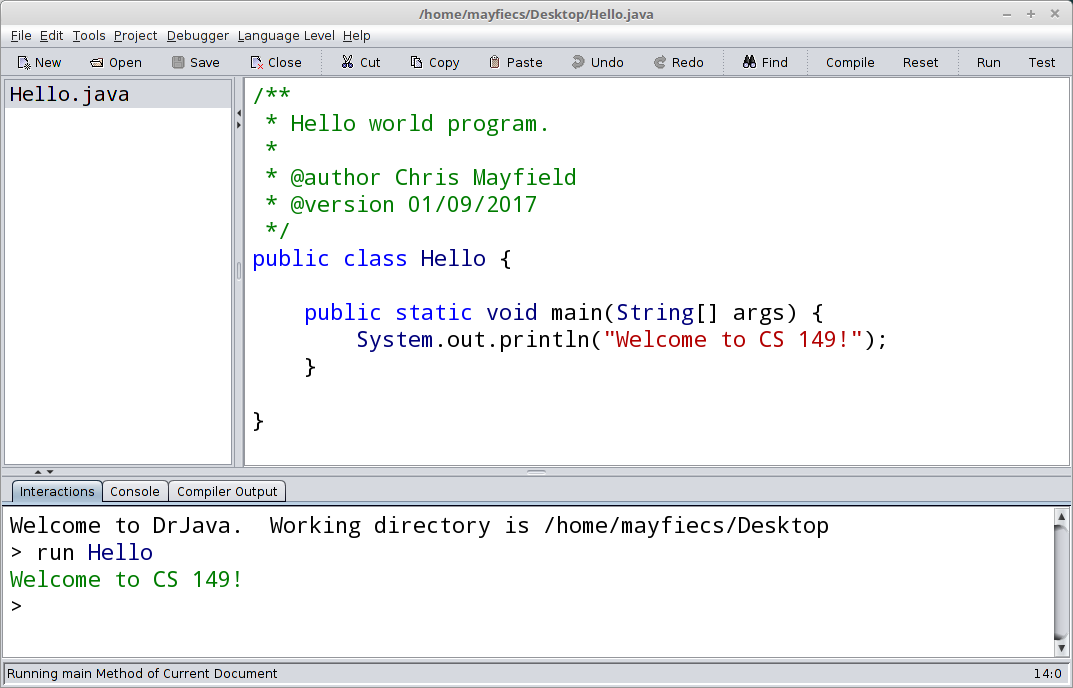
\includegraphics[height=3.65in]{drjava.png}
\end{center}


\quest{8 min}


\Q What is the name of the class?
What is the name of the file?
What directory is it in?

\begin{answer}
Class name: \texttt{Hello} ~~~
File name: \texttt{Hello.java} ~~~
Directory: \texttt{/home/mayfiecs/Desktop}
\end{answer}


\Q How many lines of code is the above program?
How many statements does it have?

\begin{answer}
The source file has 13 lines.
There is only one statement (the \java{System.out.println}).
\end{answer}


\Q What is the purpose of the first six lines?
What is the purpose of the two blank lines?

\begin{answer}
The first six lines describe what the program does and who wrote it.
The two blank lines make it easier to read the program (and are ignored).
\end{answer}


\Q Describe in your own words what \java{System.out.println} does.
Be very specific.

\begin{answer}
The \java{println} method displays a message on the screen, followed by a newline character.
When you run the \java{Hello} program, it prints a welcome message.
\end{answer}
